\subsubsection{Input Abstraction Layer}

In OpenXR, an interaction profile path defines a collection of input components (e.g., buttons, triggers, and sensors) arranged in a standardized physical configuration. This abstraction enables applications and runtime systems to coordinate action bindings independently of specific hardware implementations.

Interaction profiles generalize various input controllers, hand gestures, and other tracking systems into a unified set of action types XrActionType. These include boolean inputs, scalar values (float), two-dimensional vectors (vector2f), and pose data, which represent position and orientation in two- or three-dimensional space \parencite{openxr2024spec}.


\begin{figure}[H]
    \caption{Meta Quest 3 Touch Plus controllers}\label{fig:xr_control}
    \centering
    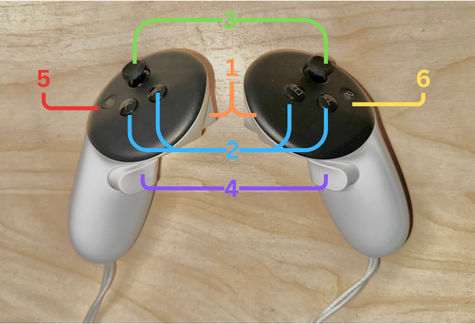
\includegraphics[width=0.8\linewidth]{img/xr.png}
\end{figure}

The hardware layout of the Meta Quest 3 Touch Plus controllers is illustrated in \cref{fig:xr_control}, while the functional mapping of each input component is summarized in \cref{table:touchPlus}.


\begin{table}[h!]
\caption{Hardware Layout of Meta Quest 3 Touch Plus Controllers}
\label{table:touchPlus}
\centering
\begin{tabular}{ll}
\toprule
Component & Description \\
\midrule
Index Trigger (1) & Analog trigger located on the front, typically used for selection or firing actions. \\
Face Buttons (2) & Left controller: X and Y buttons; right controller: A and B buttons. \\
Thumbstick (3) & Analog stick used for navigation or movement; includes a clickable button (L3/R3). \\
Grip Button (4) & Analog side button commonly used for grabbing interactions. \\
Menu Button (5) & Located on the left controller; used to open in-application menus. \\
Meta Button (6) & Located on the right controller; used to access the system-level menu. \\
Thumbrest & Capacitive surface for detecting thumb placement. \\
\bottomrule
\end{tabular}
\end{table}

Raycasting is a widely used pointing-based interaction technique in extended reality (XR), where a virtual ray is projected from an input device (e.g., a controller) into the virtual environment to enable distant object selection. The ray is typically defined by the pose of the controller, with its origin at the device position and its direction aligned with its forward orientation \parencite{mine_virtual_1995, bowman_evaluation_1997}. 

In modern XR systems such as OpenXR, raycasting is commonly implemented using pose-based input actions. Combined with discrete inputs such as the index trigger or grip button, users can effectively select and manipulate objects within a three-dimensional environment.